\documentclass[addpoints,12pt,ngerman,answers]{exam}
\usepackage[utf8]{inputenc}
\usepackage[T1]{fontenc}
\usepackage{booktabs}
\usepackage{babel}
\usepackage{graphicx}
\usepackage{csquotes}
\usepackage{paralist}
\usepackage{xcolor,siunitx}
\usepackage{listings,tikz}
\usepackage{flowchart}
\usetikzlibrary{arrows}


\definecolor{hellgelb}{rgb}{1,1,0.8}
\definecolor{colKeys}{rgb}{0,0,1}
\definecolor{colIdentifier}{rgb}{0,0,0}
\definecolor{colComments}{rgb}{1,0,0}
\definecolor{colString}{rgb}{0,0.5,0}

\pointpoints{Punkt}{Punkte}
\bonuspointpoints{Bonuspunkt}{Bonuspunkte}
\renewcommand{\solutiontitle}{\noindent\textbf{Lösung:}\enspace}
 
\chqword{Frage}   
\chpgword{Seite} 
\chpword{Punkte}   
\chbpword{Bonus Punkte} 
\chsword{Erreicht}   
\chtword{Gesamt}
\hpgword{Seite:}
\hpword{Punkte:}
\hsword{Ergebnis:}

\hqword{Aufgabe:}
\htword{Summe:}

\newcommand{\dozent}{Dr. Uwe Ziegenhagen}
\newcommand{\fach}{Klausur Informatik}
 
\pagestyle{headandfoot}
\runningheadrule \firstpageheadrule
\firstpageheader{}{}{\dozent \\ \fach}
\runningheader{}{}{\dozent \\ \fach}
\firstpagefooter{}{}{\thepage\,/\,\numpages}
\runningfooter{}{}{\thepage\,/\,\numpages}

\begin{document}

\begin{questions}
\question[5]
Schreiben Sie eine Python-Funktion, die quadratische Gleichungen der Form $-\frac{p}{2}\pm \sqrt{ \left(\frac{p^2}{4}\right)-q}$

\begin{solution}
\begin{lstlisting}[language=Python]
from math import sqrt

def solveQuad(p, q):
    partOne = -p/2
    partTwo = sqrt((-p/2)**2 - q)
    return (partOne-partTwo,partOne+partTwo)
 
print(solveQuad(1,-1))
\end{lstlisting}

\end{solution}

\question[5]
Beschreiben Sie den Aufbau der folgenden HTML-Datei.

\begin{lstlisting}[language={HTML},basicstyle=\ttfamily\small,identifierstyle=\color{colIdentifier},keywordstyle=\color{colKeys},stringstyle=\color{colString},commentstyle=\color{colComments}]
<HTML>
 <HEAD>
  <TITLE>Hallo Welt</TITLE>
 </HEAD>
 <BODY>
  Hallo LaTeX!
 </BODY>
</HTML>
\end{lstlisting}

\begin{solution}
Besteht aus mehreren Tags, der Titel lautet \enquote{Hallo Welt}
\end{solution}


\question[5] Wer hat \TeX\ erfunden?

\begin{checkboxes}
\choice John von Neumann
\choice Leslie Lamport
\CorrectChoice Donald Knuth
\choice Tim Berners-Lee
\choice Bill Gates
\end{checkboxes}

\newpage

\question[5]
Erweitern Sie den folgenden Flowchart um die BackOffice-Verarbeitungsprozesse!

\centering
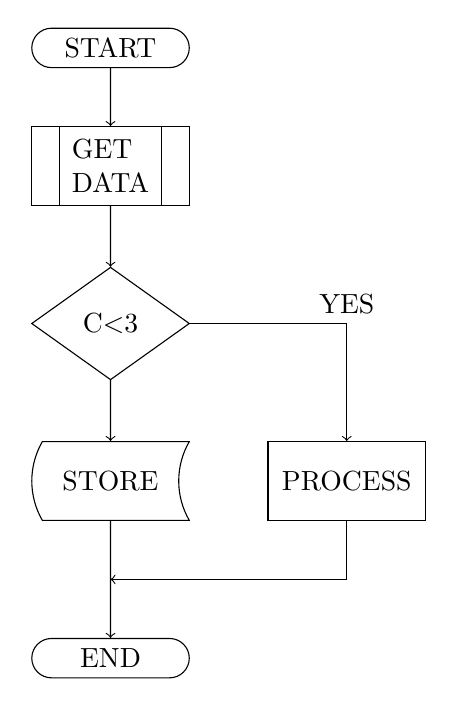
\begin{tikzpicture}
\def\smbwd{2cm}
 
\node (terminal1) at (0,0) [draw, terminal,
 minimum width=\smbwd,
 minimum height=0.5cm] {START};

\node (predproc1) at (0,-1.5) [draw, predproc, align=left,
 minimum width=\smbwd,
 minimum height=1cm] {GET\\ DATA};

\node (decide1) at (0,-3.5) [draw, decision,
 minimum width=\smbwd,
 minimum height=1cm] {C$<$3};

\node (storage1) at (0,-5.5) [draw, storage,
 minimum width=\smbwd,
 minimum height=1cm] {STORE};

\node (process1) at (3,-5.5) [draw, process,
 minimum width=\smbwd,
 minimum height=1cm] {PROCESS};

\coordinate (point1) at (0,-6.75);

\node (terminal2) at (0,-7.75) [draw, terminal,
 minimum width=\smbwd,
 minimum height=0.5cm] {END};

 \draw[->] (terminal1) -- (predproc1);
 \draw[->] (predproc1) -- (decide1);
 \draw[->] (decide1) -| node[above]{YES} (process1);
 \draw[->] (decide1) -- (storage1);
 \draw[->] (process1) |- (point1);
 \draw[->] (storage1) -- (point1) -- (terminal2);

\end{tikzpicture}\vspace*{1cm}



\end{questions}

\gradetable[h]

\end{document}